% interactcadsample.tex
% v1.03 - April 2017

\documentclass[]{interact}

\usepackage{epstopdf}% To incorporate .eps illustrations using PDFLaTeX, etc.
\usepackage{subfigure}% Support for small, `sub' figures and tables
%\usepackage[nolists,tablesfirst]{endfloat}% To `separate' figures and tables from text if required

\usepackage{natbib}% Citation support using natbib.sty
\bibpunct[, ]{(}{)}{;}{a}{}{,}% Citation support using natbib.sty
\renewcommand\bibfont{\fontsize{10}{12}\selectfont}% Bibliography support using natbib.sty

\theoremstyle{plain}% Theorem-like structures provided by amsthm.sty
\newtheorem{theorem}{Theorem}[section]
\newtheorem{lemma}[theorem]{Lemma}
\newtheorem{corollary}[theorem]{Corollary}
\newtheorem{proposition}[theorem]{Proposition}

\theoremstyle{definition}
\newtheorem{definition}[theorem]{Definition}
\newtheorem{example}[theorem]{Example}

\theoremstyle{remark}
\newtheorem{remark}{Remark}
\newtheorem{notation}{Notation}


% tightlist command for lists without linebreak
\providecommand{\tightlist}{%
  \setlength{\itemsep}{0pt}\setlength{\parskip}{0pt}}



\usepackage{hyperref}
\usepackage[utf8]{inputenc}
\def\tightlist{}


\begin{document}


\articletype{ORIGINAL RESEARCH ARTICLE}

\title{The Changing Shape of Empire: A Morphological Study of Curated
Chimú Jars and Bottles}


\author{\name{R. Alan Covey$^{a}$, Robert Z. Selden, Jr.$^{b}$, Astrid
Runggaldier$^{c}$, Nicole D. Payntar$^{a}$}
\affil{$^{a}$Department of Anthropology, The University of Texas at
Austin; $^{b}$Heritage Research Center, Stephen F. Austin State
University; Department of Biology, Stephen F. Austin State University;
and Cultural Heritage Department, Jean Monnet
University; $^{c}$Department of Art and Art History, The University of
Texas at Austin; The Mesoamerica Center, The University of Texas at
Austin; $^{d}$Department of Anthropology, The University of Texas at
Austin}
}

\thanks{CONTACT R. Alan
Covey. Email: \href{mailto:R.Alan.Covey@austin.utexas.edu}{\nolinkurl{R.Alan.Covey@austin.utexas.edu}}, Robert
Z. Selden,
Jr.. Email: \href{mailto:zselden@sfasu.edu}{\nolinkurl{zselden@sfasu.edu}}, Astrid
Runggaldier. Email: \href{mailto:astrid@austin.utexas.edu}{\nolinkurl{astrid@austin.utexas.edu}}, Nicole
D.
Payntar. Email: \href{mailto:npayntar@utexas.edu}{\nolinkurl{npayntar@utexas.edu}}}

\maketitle

\begin{abstract}
After centuries of looting along Peru's North Coast, archaeologists
acknowledge that the pottery of the Chimú Empire is one of the most
collected Andean artifacts, but also one of the most poorly understood.
Much of the enduring classificatory uncertainty comes from the
problematic provenance of most Chimú vessels, and the fact that the
distinctive blackware identified as Chimú represents the production of
workshops from across an extensive area, during periods of regional
political decentralization (CE 900-1200), imperial growth (CE
1200-1450), and foreign conquest by the Inca (CE 1450-1535) and Spanish
(after CE 1532) empires. This chapter builds on previous seriations and
field observations, using geometric morphometric analysis of a sample of
3D-scanned Chimú bottles from publicly held collections at the
University of Texas at Austin. Since Chimú bottles were formed in
workshops using molds, variations in vessel shape can serve as
indicators of variable practices. We compare a sample of common Chimú
blackware bottles with a sample of \emph{Inca-Chimú} vessels that carry
features typical of the short Inca occupation of the North Coast.
Differences between the two vessel forms offer new lines of evidence
that can guide new interpretations of the imperial history of Peru's
North Coast.
\end{abstract}

\begin{keywords}
Computational Archaeology; Museum Studies; Digital Humanities;
Non-Western Art History; STEM; STEAM
\end{keywords}

\hypertarget{the-collecting-history-of-an-imperial-ware}{%
\section{The Collecting History of an Imperial
Ware}\label{the-collecting-history-of-an-imperial-ware}}

The distinctive blackware pottery of the Chimú Empire of Peru's north
coast is among the most intensively collected Andean styles, but also
one of the least-defined. Thousands of well-preserved vessels occupy the
shelves of museums in South America, North America, and Europe, from the
vast collections of famous institutions like Berlin's Ethnologisches
Museum to local museums that possess a single vessel of unknown
provenance. It is impossible to know when Europeans first began to
collect Chimú blackwares, although published illustrations date back as
far as the early eighteenth century \citep[Figure 1]{RN11149t}.

\emph{\textbf{{[}Figure 1 about here. Frézier image of north coast
blackwares in an image of ``Inca'' culture{]}}}

By that time, Spaniards had already been plundering Peru's coastal
huacas for nearly two centuries, mining them to extract the gold and
silver found in rich burials. Nineteenth-century collecting shifted the
emphasis from precious metals, toward the recovery of well-preserved
human crania that could be used to buttress European beliefs in their
own racial superiority. Over time, Chimú ceramics (and other artifacts)
were caught up in the new collecting regime as public museums grew in
the global North \citep[50-51]{RN11150}. By the early twentieth century,
large numbers of unauthorized diggers were working full-time excavating
tombs at Chan Chan, the ruined Chimú capital \citep[15]{RN11151}, and
Chimú pottery could be purchased from shops in the Peruvian city of
Trujillo (Figure 2). \citet[570]{RN11152} noted at that time that the
blackware vessels of Peru's north coast were already ``very well
represented in most ethnographic collections.'' Since then, coastal
blackwares have continued to be excavated and trafficked by illicit
diggers who target more valuable metal artifacts and polychrome textiles
\citep{RN11153}, and today they can be readily found at internet auction
sites for modest prices.

\emph{\textbf{{[}Figure 2 about here. Map of the north coast of
Peru{]}}}

The history surrounding the collection of Chimú blackwares helps to
explain why this ubiquitous artifact class remains poorly understood by
professional archaeologists. When viewed as a byproduct of collecting
activities that unfolded over almost a half millennium, the Chimú
ceramic corpus can be seen for what it is: an ambiguous assemblage of
mostly orphaned objects. Almost all Chimú vessels lack a detailed
archaeological provenience, and the chain of ownership for most museum
pieces can rarely be traced back to Peru. Because most ``Chimú'' vessels
cannot be affiliated to a particular context in coastal Peru, their
identification derives from their stylistic attributes, even though some
of the earliest Chimú ceramics documented in archaeological excavations
appeared at the Inca site of Machu Picchu \citep[269]{RN7063} and the
coastal creation shrine of Pachacamac, two sites that lie well beyond
the political control of the Chimú Empire \citep[756]{RN11154}.

This contextual ambiguity intersects with a classificatory problem for
Andean archaeology. Many treat Chimú pottery as typical of the Late
Intermediate Period (CE 900-1476) on the north coast of Peru, a huge and
undifferentiated period during which the Chimú polity established its
capital and local dominion in the Moche Valley, carried out multiple
waves of imperial expansion to the north and south, and fell under the
hegemony of Inca imperial rule (CE 1476-1532). Excavators have noted
that similar blackwares continued to be produced during the half century
of Inca rule, and into the earliest years of the Spanish colonial
period. Without knowing when and where a particular museum object comes
from, archaeologists have faced difficulties in subdividing Chimú
pottery into phases and substyles, which would enable researchers to
study changes and variations within the overall assemblage.

\hypertarget{early-archaeological-classifications}{%
\subsection{Early Archaeological
Classifications}\label{early-archaeological-classifications}}

From early on, classifications of Chimú ceramics focused on vessel
attributes. \citet[652-654]{RN11152} noted that coastal tombs had
yielded ``infinite'' formal variations of blackware pots now found in
museum collections. He placed these into five principal categories: (1)
globular vessels with rectangular fields of low-relief decoration; (2)
geometric vessels (cuboid, ellipsoids, ovular); (3) phytomorphic vessels
shaped like squash or fruits; (4) zoomorphic vessels representing a
broad range of fauna; and (5) anthropomorphic vessels. This
classification emphasized aesthetic characteristics of vessel shape,
rather than the kinds of formal and functional differences seen in later
typologies, and Beuchat acknowledged the diversity found within each of
his categories, especially the phytomorphic, zoomorphic, and
anthropomorphic vessels. Without any provenience information to guide
his analysis, Beuchat did not attempt to seriate Chimú pottery or to
distinguish regional variations.

In 1926, Alfred Kroeber made the first concerted effort to describe
different phases of Chimú ceramic production, based on a brief visit to
the Trujillo area that he made as part of a Field Museum expedition to
the central coast. Kroeber noted previous efforts by \citet{RN11154} to
differentiate between early and late ceramics from Trujillo, which could
be tied to the Moche site of Huaca de la Luna/Huaca del Sol and the
Chimú capital of Chan Chan. Kroeber used the term \emph{Late Chimú} to
refer to Trujillo area blackwares that sometimes were found with Inca
ceramics, a designation that encompasses Late Intermediate Period (CE
900-1400s), Inca (CE 1400s-1530s) and some early Colonial pottery. Based
on provenance information that recorded the district where some Late
Chimú vessels originated, \citet[11]{RN11151} identified a broad
distribution that stretched from Piura to Casma, with some vessels found
as far south as the Nasca drainage. To build a typology and sequence of
Late Chimú vessels, he studied the pottery from several collections that
he purchased in Trujillo on behalf of the Field Museum.

Kroeber's shape typology for Late Chimú pottery discusses vessels that
were common in Moche and Chimú assemblages, and he lists
\citep[22]{RN11151} about a dozen Late Chimú shapes, including
stirrup-mouth vessels, double jars, double-spout vessels, head-and-spout
vessels, figure-and-spout vessels, globular bowls, lipped pots (with and
without handles), jars with flaring mouth, flat-handled jars, and jars
with tapering spouts. The list of shapes also includes Inca narrow-mouth
jars (\emph{aryballus}) and cups (\emph{kero}) in the Late Chimú
assemblage. In his decorative analysis of vessels in private
collections, \citet[27-28]{RN11151} identified the \emph{face vase} and
\emph{rotund figure jar} as additional shapes found in the assemblage.
The discussion of Late Chimú blackware recorded the relative abundance
of the most common shapes found in two private collections that he saw
while visiting Trujillo. The Mansiche and Jacoms collections comprised
more than 200 vessels, but Kroeber estimated that hundreds of
utilitarian pots, plates, and jars had been \emph{rejected} by the
collectors when they purchased vessels from the huaqueros who excavated
them near Chan Chan.

In his study of collected ceramics from Trujillo, Kroeber established
the outline of a shape typology for Chimú blackware vessels, although it
was not a comprehensive representation of ceramics in use on the north
coast during the periods of Chimú, Inca, and Spanish imperial expansion.
Building on the earlier observations of the high degree of diversity
seen in Chimú blackwares, Kroeber made some important observations that
inform subsequent studies. First, this pottery is widely distributed
along the north coast of Peru, although \citet[97]{RN11155} argued for
strong continuity between regions, which would suggest that regional
variations account for little of the overall diversity in the Chimú
assemblage. Second, he noted that blackwares were strongly associated
with mortuary contexts, and such pottery was not commonly seen on the
surface of the urban core of Chan Chan. Such vessels were thus more
indicative of Chimú funerary practices than everyday life. Finally,
Kroeber described how the private collections that local dealers
assembled and sold to museums were already curated in a way that
eliminated certain vessel shapes, so that museum collections could be
considered representative of the original mortuary assemblage. As
Kroeber noted \citep[95]{RN11155} in a later visit to the north coast,
one Trujillo collector ``refused to purchase from the huaqueros most of
the unhandled jars, exceptions being made in favor of effigy pieces, or
occasional plain ones when several vessels were bought in a lot in order
to acquire one or two attractive ones.''

\hypertarget{attempts-at-seriation}{%
\subsection{Attempts at Seriation}\label{attempts-at-seriation}}

In the years following Kroeber's work, analysis of Chimú ceramics
continued to be oriented around the integration of regional Andean
sequences, and the pottery of the Chimú Empire continued to be discussed
alongside Moche ceramics that were considered to be Early Chimú
\citep{RN11156,RN11157}. It was not until the 1960s that a concerted
effort was made to move beyond the master sequence, to developed a more
fine-grained description of the assemblage associated with the Chimú
Empire as it developed, expanded, and fell under Inca and Spanish
dominion. In 1966, Harry Scheele and Thomas Patterson published a
``preliminary seriation'' of Chimú ceramics. They noted
\citep[15]{RN11158} that one reason that so little work had been done to
classify such material was its abundance: ``probably no other pottery
style from the Americas is so well represented on the shelves of museums
and private collectors throughout the world.''

As noted already, this prevalence was remarked on almost 50 years
earlier, the result of large-scale collections acquisitions that major
museums had engaged in since the late 1800s (e.g., Květinová
2011:65-66). But Chimú pottery continued to flow into established museum
collections, and to be sought as new museums were established (see Mowat
1988 for an example of donation and accessioning practices).
Collection-building accelerated as new museums were founded after World
War II and continued with limited constraints until after 1970, when the
UNESCO Convention regarding cultural property established guidelines
that gradually altered legal standards and ethical practices surrounding
collecting (Gerstenblith 2013). Although some museums continued to send
curators to Peru to purchase from antiquities dealers, a cursory review
of museum records reveals that many new accessions came as gifts from
individual donors, who provided little or no provenance information. For
example, the Metropolitan Museum of Art received a feline bottle
(64.228.17) from Nathan Cummings in 1964, who had purchased the vessel a
decade earlier from a collector in Buenos Aires. The piece was one of
more than 1000 artifacts that Cummings is credited with donating to the
museum. The Cleveland Museum of Art, founded in 1913, also built its
collections through donations, including a blackware jar (1959.333)
given by William Ellery Greene in 1959. It was the only Andean artifact
given to the museum by the donor.

Building on preliminary work by Pedro Rojas Ponce and Dorothy Menzel,
Sheele and Patterson (1966) compared illustrations from the published
literature with vessels from Peru's Museo Nacional de Antropología y
Arqueología and Harvard University's Peabody Museum of Archaeology and
Ethnology. They created a preliminary seriation of Chimú ceramics from
the end of the Middle Horizon to the early Colonial Period,
distinguishing seven different phases based on the identification of
different vessel shapes, decorative elements, and firing
characteristics. Although the seriation was developed to build a more
fine-grained relative chronology, the small sample sizes of some phases
presented interpretive challenges. For example, the fourth phase
\emph{Lambayeque}, was based on seven vessels from a single grave in the
Lambayeque Valley, located approximately 175 km to the north of Chan
Chan, and probably reflects regional ceramic diversity more than a
distinct period of Chimú production in the Moche Valley. Other phases
were based on small sample sizes and vessels with limited provenance
information. One important distinction in the Scheele and Patterson
seriation was between Chimú ceramics of the late LIP (Chimu Phase T-1)
and those from the time of the Inca occupation (Chimu Phase T-2). The
former was defined based on the prevalence of stirrup-spout vessels and
the \emph{less carefully made} production of mold-produced vessels that
seemed to represent a more restricted set of shapes than the preceding
phase (Trujillo Phase T-2). The Chimú-Inca phase maintained elements of
existing ceramic production, adding features from Inca vessel shapes.
Scheele and Patterson note (1966:24) that this phase seems to be
distributed beyond earlier Chimu political boundaries and economic
networks---it has been identified on the south and central coast and in
the Cuzco region. Overall, Scheele and Patterson's work clarifies how
some vessel shapes developed over time, making it possible to assign
provenienced gravelots to more specific late prehispanic periods. It
also identified some important aspects of production practices and
hybridity that have been important for subsequent archaeological
fieldwork.

\hypertarget{field-archaeology-and-the-reconstruction-of-production-practices}{%
\subsection{Field Archaeology and the Reconstruction of Production
Practices}\label{field-archaeology-and-the-reconstruction-of-production-practices}}

Although the first attempts at defining Chimú ceramics within a broader
north coast sequence utilized museum collections, archaeological
excavations have increasingly contributed to the reconstruction of
ceramic production practices. In the mid-20th century, excavators turned
to cemeteries as a source of well-provenienced vessels that could be
used to elaborate the regional sequence (e.g., Collier 1955; Willey
1947). Such work represented only a miniscule proportion of Chimú
ceramics that were being dug up at that time, most of which were
obtained by huaqueros whose illicit work supplied private collectors and
museums around the world. Studies of whole vessels concluded that the
use of molds increased in late prehispanic periods on the north coast
(Collier 1955), and by the 1960s, some researchers had identified molds
and matrices in the pottery collections acquired by some museums (e.g.,
Grossman 1969-1970; Thompson 1963). Such work constituted an important
step toward moving from straightforward aesthetic considerations to
questions about the production and consumption of Chimú ceramics, but it
remained rooted in mortuary collections that did not focus on evidence
of production practices.

At the end of the 1960s, Moseley and Mackey's Chan Chan-Moche Valley
Project (1969-1975) began to increase the intensity of professional
archaeological research, with regional survey work in the lower Moche
Valley and mapping and excavations at Chan Chan and other nearby sites.
While not focused on cemetery sites, this project and related studies
encountered additional mortuary contexts with well-preserved ceramics
(see Donnan and Mackey 1978). It was not until the 1990s, however, that
archaeologists began to identify loci of ceramic production based on the
presence of overfired sherds, molds and matrices, stamps, tools, kilns,
and other evidence (Donnan 1997; Hayashida 1999; Mackey 2003; Mackey and
Sapp 2021; Tschauner 2006, 2009). Some of the workshops reflect ceramic
production practices during the preceding era of Chimú imperial
expansion, whereas others were in use during the Inca occupation of the
north coast. Surface collections and excavations in production areas
generated multiple lines of material evidence, including large numbers
of potsherds that could not easily be assigned to the diverse array of
shapes identified in collection-based classifications.

The study of Chimú and Chimú-Inca pottery workshops has focused on two
central themes: specialization and cultural (dis)continuity under
foreign rule. These issues were nascent in many of the earlier
collection-based studies, but the careful excavation and analysis of
production contexts added invaluable evidence to the discussion. Molds
and matrices encountered at workshops indicate that multiple vessel
parts were mass-produced and had to be assembled following a specific
sequence, which Tschauner (2006:179) interprets as evidence of
specialized production during Chimú times. Tschauner's excavations at
the Pampa de Burros workshop in the Lambayeque Valley identified heavy
use of vertical half-molds to produce jars, canteens or flasks, bottles,
and ollas---virtually all of the shapes that were used by Chimú-era
settlements in the surrounding valley (2006:182). He sees the local
potters as relatively unskilled producers who relied on more adept
makers of ceramic molds, and whose \emph{market-oriented} work could
flexibly adapt to consumer preferences (2006:183-185). Levine (2011)
builds on this idea, noting that some of the variability seen in the
Chimú assemblage could come from ceramic producers \emph{mixing and
matching} molds for different vessel parts and adornments to produce new
combinations.

For the Inca period, scholars acknowledge a degree of continuity in
local potting practices, but also some significant changes. At Tambo
Real and La Viña in the Leche Valley, Hayashida (1999) notes the
continuity of local practices for shaping vessels (press molds, paddle
and anvil) and firing. While local jar shapes persisted in Inca times,
she observes the presence of a mold for an Inca flared jar neck
(1999:345), which could be added to jars that were shaped using local
press molds. Overall, Hayashida sees little evidence of Inca
\emph{retraining} of Chimú potters.

Other Inca-Chimú workshops in the Jequetepeque Valley provide evidence
that practices varied at different production locations. Donnan's
(1997:32-35) surface collections at Cañoncillo encountered dozens of
mold fragments, most of which were for shaping the bottom and top
hemispheres of ollas. Donnan identified molds for shaping jars along a
vertical axis, and for producing bottles, including the distinctive Inca
``aryballoid'' shape. Although he reports that no molds appeared for
shaping handles or rims, there were molds for producing stirrup spouts,
as well as for humans, birds, and other animals. The production evidence
from this site suggests that while some vessels were largely shaped
using molds, some elements were hand-formed and showed variations
suggesting the work of multiple potters. At the Inca administrative
center of Farfán, Mackey (2004:336-338) excavated a small workshop that
produced large jars (tinajas) for brewing or storage, using the
paddle-and-anvil technique. Finally, the excavation of three workshop
patios at El Algarrobal de Moro, a lower-order Chimú administrative
center, encountered 25 mold fragments, including molds for a stirrup
spout vessel and a miniature jar (Mackey and Sapp 2021:21-22).

\hypertarget{technological-approaches-to-chimuxfa-ceramics}{%
\subsection{Technological Approaches to Chimú
Ceramics}\label{technological-approaches-to-chimuxfa-ceramics}}

The accumulation of excavation assemblages with Chimú blackwares
occurred as archaeologists developed new approaches to the study of
ancient pottery. Archaeologists often find it difficult to map the
shape-based categorizations developed from whole vessels in museum
collections onto the broken fragments they encounter in excavation
contexts other than tombs. Middens and house floors typically contain an
assemblage that is not fully represented in the corpus of collected
vessels, which has been biased toward mortuary offerings and shaped by
the aesthetic values of dealers and collectors. Field researchers have
used stylistic approaches to assign rough dates from the relative
sequence, but the anthropological analysis of excavated pottery has
inspired archaeological ceramicists to focus on the social practices
underlying the production, distribution, use, and discard of pottery.
The shift from style to technology has coincided with the introduction
of methods to study the composition of clays, tempers, and pigments used
for produce archaeological ceramics.

Given the acknowledged challenges in classifying Chimú vessels, it is
not surprising that recent ceramic studies have embraced technological
analyses, including petrography (Krzanowski and Pawilowski 1980),
neutron activation, X-ray diffraction, X-ray fluorescence,
particle-induced X-ray emission (Cunha Lima 2010), and Mössbauer
spectroscopy (Tschauner and Wagner 2003). Despite such work, Shimada and
Wagner (2019) argue that the reconstruction of the chaîne opératoire for
north coast blackwares remains incomplete. It should be noted that many
of the techniques used to reconstruct production practices rely on
samples of potsherds that can be removed to the laboratory, and
potentially altered or destroyed in the process of analysis. More
recently, researchers have brought non-destructive techniques such as CT
scans (Wauters 2016) and linear morphometric analysis (Květinová 2011)
to the study of museum collections. This work emphasizes the variability
found in different vessel categories, as well as the reconstruction of
productive processes, including the use of molds to manufacture vessel
bodies and other elements.

\hypertarget{d-scanning-and-geometric-morphometrics-analysis-of-chimuxfa-pottery}{%
\subsection{3D Scanning and Geometric Morphometrics Analysis of Chimú
Pottery}\label{d-scanning-and-geometric-morphometrics-analysis-of-chimuxfa-pottery}}

After a century of classifying Chimú ceramics and reconstructing their
production and social uses, archaeologists have yet to bring order to
the \emph{infinite} diversity of the museum assemblage, but they have
developed important questions for empirical analysis. Rather than
attempting to fit Chimú vessels into a neat taxonomy, researchers have
drawn attention to the different factors influencing diversity in late
prehispanic blackwares. Blackware ceramics were produced over several
centuries and across a broad stretch of the north coast, and a
significant degree of variation comes from the practices of individual
potters at different workshops, who were producing different vessels to
meet the changing aesthetic tastes of coastal consumers. There appear to
have been differences in the organization of pottery workshops, and some
producers relied more on the use of molds and matrices than others. It
is not presently clear who designed and produced molds and matrices, or
how broadly used and consistently replicated such production templates
were. A fine-grained three-dimensional study of vessel bodies and key
elements known to have been molded in some instances (e.g., stirrup
spouts) could quantify the amount of variation seen in well-preserved
vessels, contributing to the discussion of how hierarchical and
centralized Chimú ceramic production was beyond the local workshop.

Previous analyses have also noted variable degrees of continuity and
change seen in the production of ceramics during the period of Inca
hegemony on the north coast. Local potters continued to produce
blackwares using many of the same techniques and tools, but they also
incorporated new vessel shapes and elements (e.g., flaring jar rims)
that were distinctly Inca. Chimú-Inca pottery is often classified
qualitatively, but a quantitative analysis of Inca vessel features that
appear on such pottery would make it possible to address questions of
hybridity, including the degree of foreign influence and the potential
resistance of potters working in specific workshops to provide pottery
for populations that experienced Inca imperial dominance in different
ways.

These two questions can be addressed using three-dimensional data from
well-preserved vessels, an approach that presents logistical challenges.
To date, Wauters (2016) has used CT scans and X-ray radiography to study
16 stirrup-spout bottles from the Royal Museums of Art and History of
Brussels and the Ethnography Museum of Geneva. To produce the scans, the
vessels had to be removed from the museums and transferred to hospitals
where the necessary equipment could be accessed. While generating
high-resolution data, funding constraints and curatorial policies would
make it difficult to conduct such research with large sample sizes. As
an alternative, portable high-resolution 3D scanning equipment can be
brought into museums to scan collections in situ, using the resulting
data for geometric morphometric analysis. Between 2018 and 2020, we
conducted exploratory research on Chimú ceramics in two collections
using this approach.

\hypertarget{collections-and-research-ethics}{%
\subsection{Collections and Research
Ethics}\label{collections-and-research-ethics}}

For our broader study, we scanned \#\#\#\# prehispanic ceramic vessels
from two collections that reflect the broader history of collecting and
curating Chimú ceramics. Our first collection was the Art and Art
History Collection (AAHC), a modest sized collection that accumulated
haphazardly at the University of Texas at Austin as numerous individuals
donors gave the university artifacts that had little or no provenance
information. The ancient pottery now in the AAHC was previously curated
by the Texas Memorial Museum, which transferred them to the department
of Art and Art History in 2004 as the museum implemented new curatorial
priorities. In 2018, we scanned 112 Andean vessels from the AAHC
collection. The data presented here come from a sample of Chimú bottles
(n=23) and jars (n=16) from the UT collection. \emph{\textbf{{[}Astrid:
How many Andean vessels overall in the collection, and how much Chimú?
Should we include a table of the samples here, with as much provenance
info as we can find?{]}}}

As a second collection, we also worked with a large museum sample that
was acquired in Peru by a professional archaeologist the early days of
museum collecting. The Bandelier Collection at the American Museum of
Natural History consists of nearly 8,000 Andean artifacts from Peru and
Bolivia. The Swiss-American archaeologist Adolph Bandelier acquired
these pieces as part of his 1890s Andean expedition, which was initially
funded by Henry Villard. Bandelier visited the Trujillo area in 1893,
where he sketched the ruins of Chan Chan and acquired more than 400
Chimú vessels and other artifacts that were accessioned by the museum.
Although the records of Bandelier's expedition remain unpublished, the
collection offers a large sample size of vessels that were collected at
the same time, during a period of archaeological collecting when dealers
were less attuned to the targeted collecting that Kroeber observed a
generation later. In 2020, we scanned \#\#\# Chimú, Inca, and Chimú-Inca
ceramic vessels at the AMNH.

The exploratory nature of the work also raised ethical considerations
regarding work with museum collections. Archaeologists have intensified
their work with museum collections in recent years, and the
consideration of whether to conduct such research are as important as
the logistical questions of how to accomplish the work. The ethical
principles of the Society for American Archaeology highlight the values
of stewardship and public responsibility---it is important for
archaeologists to care for the material record, and also to share
information about it with the public---identifying ``public education
and outreach'' as significant. From this perspective, the
non-destructive and museum-based work of 3D scanning presented little
risk to the artifacts being analyzed, and our research was designed to
be available to the public. When working with the AAHC vessels, we
developed an educational component, including a small class of UT
undergraduates in the lab-based collection of linear measurements of the
vessels being scanned. That supervised research provided a diverse group
of undergraduates with artifact analysis, while also teaching them about
the loss of heritage and scientific knowledge that accompanies the
collection of antiquities.

While the careful study and public reporting of museum collections is
consistent with professional ethics in Americanist archaeology, the SAA
also identifies a potential ethical concern in doing so: the
commercialization of the archaeological record. The SAA clearly states
that ``Archaeologists should therefore carefully weigh the benefits to
scholarship of a project against the costs of potentially enhancing the
commercial value of archaeological objects. Whenever possible they
should discourage, and should themselves avoid, activities that enhance
the commercial value of archaeological objects, especially objects that
are not curated in public institutions, or readily available for
scientific study, public interpretation, and display.'' As described
above, Chimú blackware pottery is an artifact class that was heavily
collected in the past, and it is openly sold today by galleries and
internet vendors. As Atwood (2004:22-23) notes, huaqueros, dealers, and
collectors are no longer interested in trafficking Andean ceramics,
especially mass-produced wares like those of the Chimú Empire. Our work
with publicly-held collections poses little risk of increasing the
present commercial value of Chimú ceramics, while its public discussion
of the losses that accompany undocumented excavations and illicit
collection constitutes a benefit that outweighs any associated risks.

\hypertarget{methods-and-results}{%
\section{Methods and Results}\label{methods-and-results}}

Linear shape variables\ldots{} (Figure \ref{fig:linear}).

\begin{figure}\centering
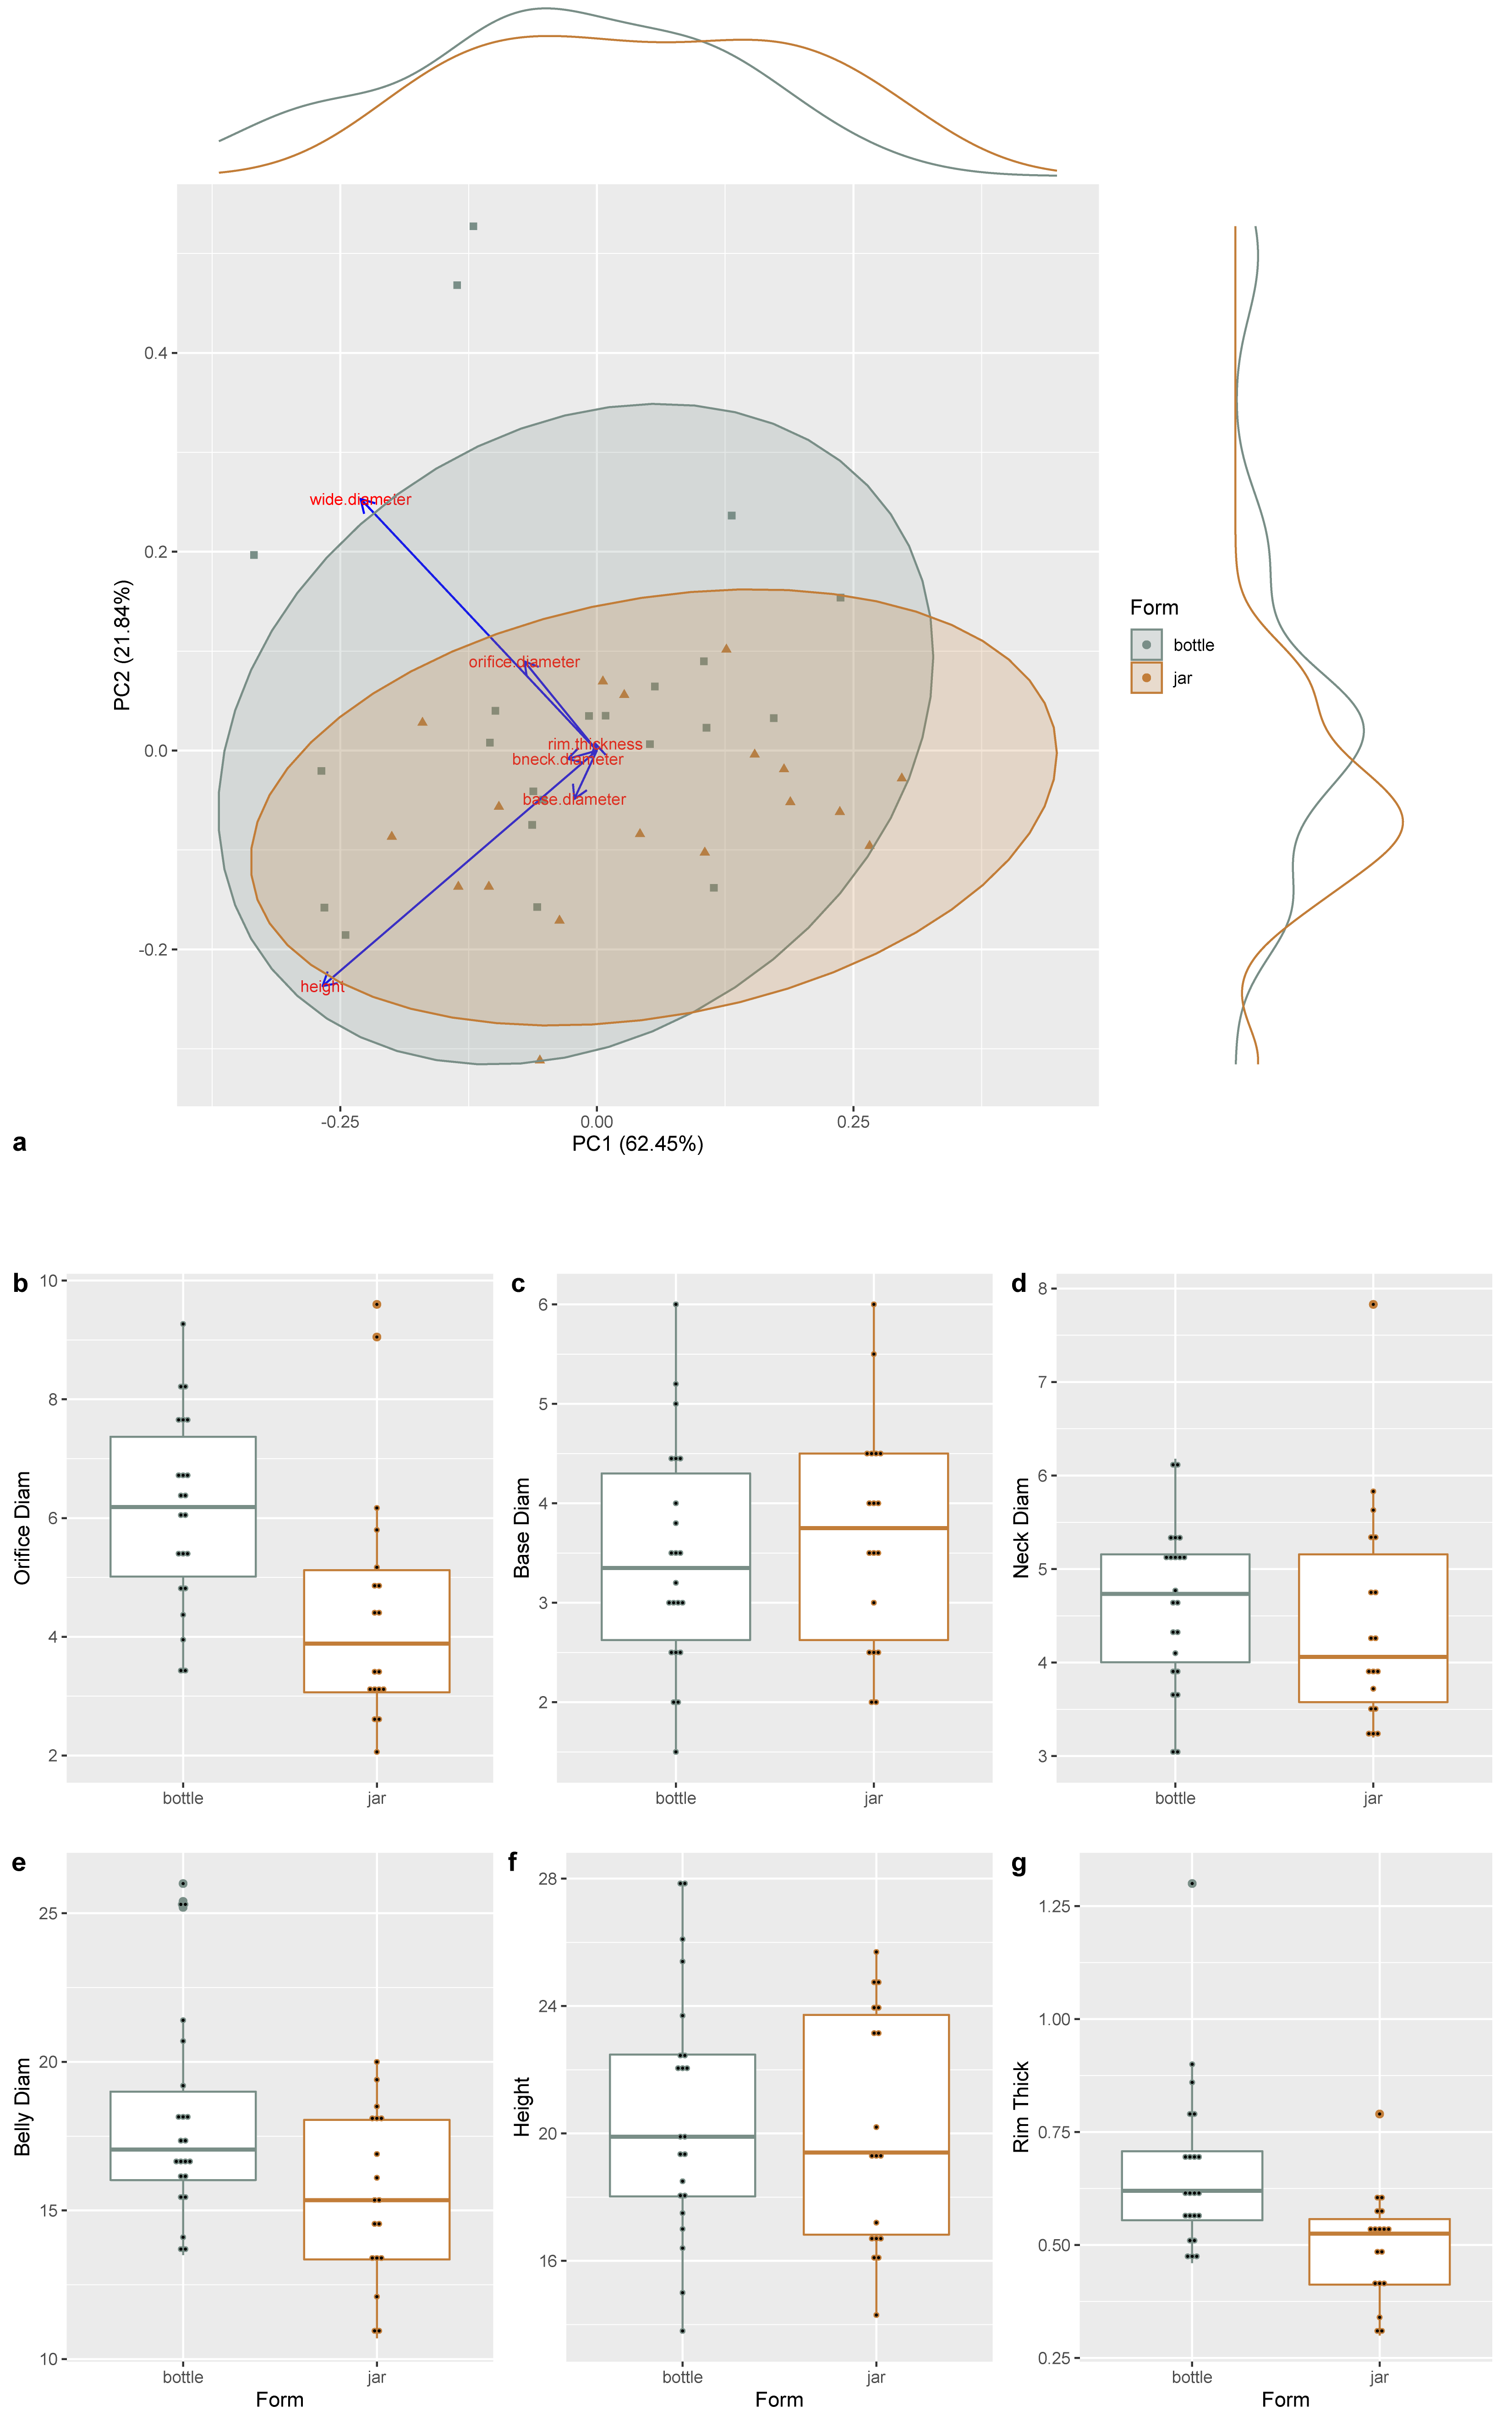
\includegraphics[width=\linewidth]{figs/linear.fig.png}
\caption{Plots of a, PCA; b, orifice diameter; c, base diameter; d, neck diameter; e, belly diameter; f, height; and g, rim thickness for linear metrics.}
\label{fig:linear}
\end{figure}

\hypertarget{geometric-morphometrics}{%
\subsection{Geometric morphometrics}\label{geometric-morphometrics}}

During the collections research, vessels were scanned with a Creaform
GoSCAN 20 at a 0.5mm resolution in VXelements. Scanner calibration was
optimized prior to each scan, with positioning targets required for
increased accuracy, and shutter speed reconfigured in each scanning
instance. Clipping planes were established to reduce the amount of
superfluous data collected, and the final mesh was rendered following
application of the clean mesh function in VXelements. This process
removed isolated patches, self-intersections, spikes, small holes,
singular vertices, creased edges, narrow triangles, outcropping
triangles, narrow bridges, and non-manifold triangles prior to export as
an ASCII stl file. The stl was subsequently imported to R where each
mesh was subjected to an automated post-processing routine using the
\texttt{Rvcg} package to detect and correct any abnormal poly-faces in
advance of performing a global remesh to improve mesh quality
\citep{RN8497}. The final meshes were then imported to Geomagic Design X
(Dx) for landmarking.

\hypertarget{alignment-and-reference-geometry}{%
\subsubsection{Alignment and reference
geometry}\label{alignment-and-reference-geometry}}

Following transfer to Dx, each mesh will be subjected to an additional
quality check to eliminate non-manifold poly-vertices, folded
poly-faces, dangling poly-faces, small clusters, small poly-faces,
non-manifold poly-faces, crossing poly-faces, and small tunnels. Due to
the paucity of homologous landmarks on cultural artefacts
\citep{RN8521}, reference geometry will be constructed around each
vessel in a manner that yields a replicable configuration of nine
landmarks, and 46 equidistant semilandmarks along the widest vessel
profile, with notable similarities to previous landmark configurations
\citep{RN7039,RN7925,RN8071,RN8361,RN8967,RN8375}, which largely follow
\citet{RN5700}.

The first component of reference geometry added was a reference vector.
A sampling ratio of 100 percent was used to apply the reference vector
on a revolving axis, after which a reference point was added by
projecting it atop the mesh surface where it intersects with the
reference vector at the point that the vector exits the base of the
vessel. A reference plane was inserted using the pick multiple points
function, by adding a series of 10 points around the circumference of
the bottle's base. Each element of reference geometry (vector, point,
and plane) was subsequently used in an interactive 3-2-1 alignment where
the vessel was aligned to a global origin, orienting it in 3D space
where it sits upright atop a planar surface (assumed to be the intent of
the maker). Following alignment, the reference plane and point were
deleted.

The widest vessel profile is defined as the location on a mesh that lies
farthest from the central point where the reference vector exits the
vessel base while oriented atop the planar surface. To identify that
location, a mesh sketch was generated with the planar method using the
plane at the base of the vessel to identify and sketch the widest vessel
circumference. By using the plane located at the base of the vessel for
the sketch, the point at which the reference vector exits the mesh
remains linked to the remainder of the reference geometry. A circle was
then sketched using the vector as the centre, extending outward until
the whole of the vessel fit within. Using a mesh sketch, a cylinder
(surface) was extruded around the full extent of the vessel. The
accuracy analyser in Dx was used to identify the point on the vessel
with the lowest deviation from the extruded surface, and a plane
(MPlane) was inserted coplanar to the vector and oriented to the widest
point, bisecting the vessel at its' widest profile.

Using the MPlane as the basis for a second sketch, a spline was
populated for the entirety of the silhouetted profile. That spline was
subsequently split at the location of the horizontal tangents and the
remaining sections that continued into the bottle interior were deleted.
The second split was added at the intersection of the spline and
reference vector (centre of base). Four additional splits were then
added at the juncture of the base/body and body/neck on each side of the
vessel at the points of highest curvature. The point of highest
curvature used to split the spline is identified using the curvature
function in Dx, and does not represent an arbitrary location.

\hypertarget{landmarks-and-semilandmarks}{%
\subsubsection{Landmarks and
semilandmarks}\label{landmarks-and-semilandmarks}}

Seven landmarks and 38 semilandmarks segregate each vessel into two
discrete components corresponding with the rim/neck, body/base.
Landmarks and semilandmarks were populated along a spline across the
vessel profile that included no abstraction/s associated with appliqued
sculptural elements. Application of landmarks and semilandmarks began on
the side of the vessel profile determined to include the widest vessel
profile. Each component was isolated using a series of spline splits,
where landmarks were later placed followed by a series of equidistant
semilandmarks. Spline splits occur at the horizontal tangent at the rim,
the point of highest curvature at the intersection of the neck and body,
the point of highest curvature at the intersection of the body and base,
and at the only intersection of the reference vector and spline at the
center of the base. The constellation of landmarks and equidistant
semilandmarks used in this study draws influence from the characteristic
points and tangents employed in the study of aesthetic measure by
\citet{RN5700}, as well as a selection of studies that followed
\citep{RN8103,RN8104}.

\hypertarget{generalised-procrustes-analysis}{%
\subsubsection{Generalised Procrustes
Analysis}\label{generalised-procrustes-analysis}}

Landmark data were aligned to a global coordinate system
\citep{RN8477,RN7502,RN11622,RN11623,RN11563}, achieved through
generalised Procrustes superimposition \citep{RN11138,RN478,RN1646} in R
using the \texttt{geomorph} and \texttt{RRPP} packages
\citep{RN1655,RN11775,RN11530,RN1774,RN9565}. Procrustes superimposition
translates and rotates the coordinate data to allow for comparisons
among objects, while also scaling each biface using unit-centroid
size---the square root of the sum of squared distances from each
landmark to the specimen's centroid
\citep{RN11139,RN11140,RN11564,RN478}. The \texttt{geomorph} package
uses a partial Procrustes superimposition that projects the aligned
specimens into tangent space subsequent to alignment in preparation for
the use of multivariate methods that assume linear space (Figure
\ref{fig:gpa}) \citep{RN11141,RN11142,RN1646,RN11563}.

\begin{figure}\centering
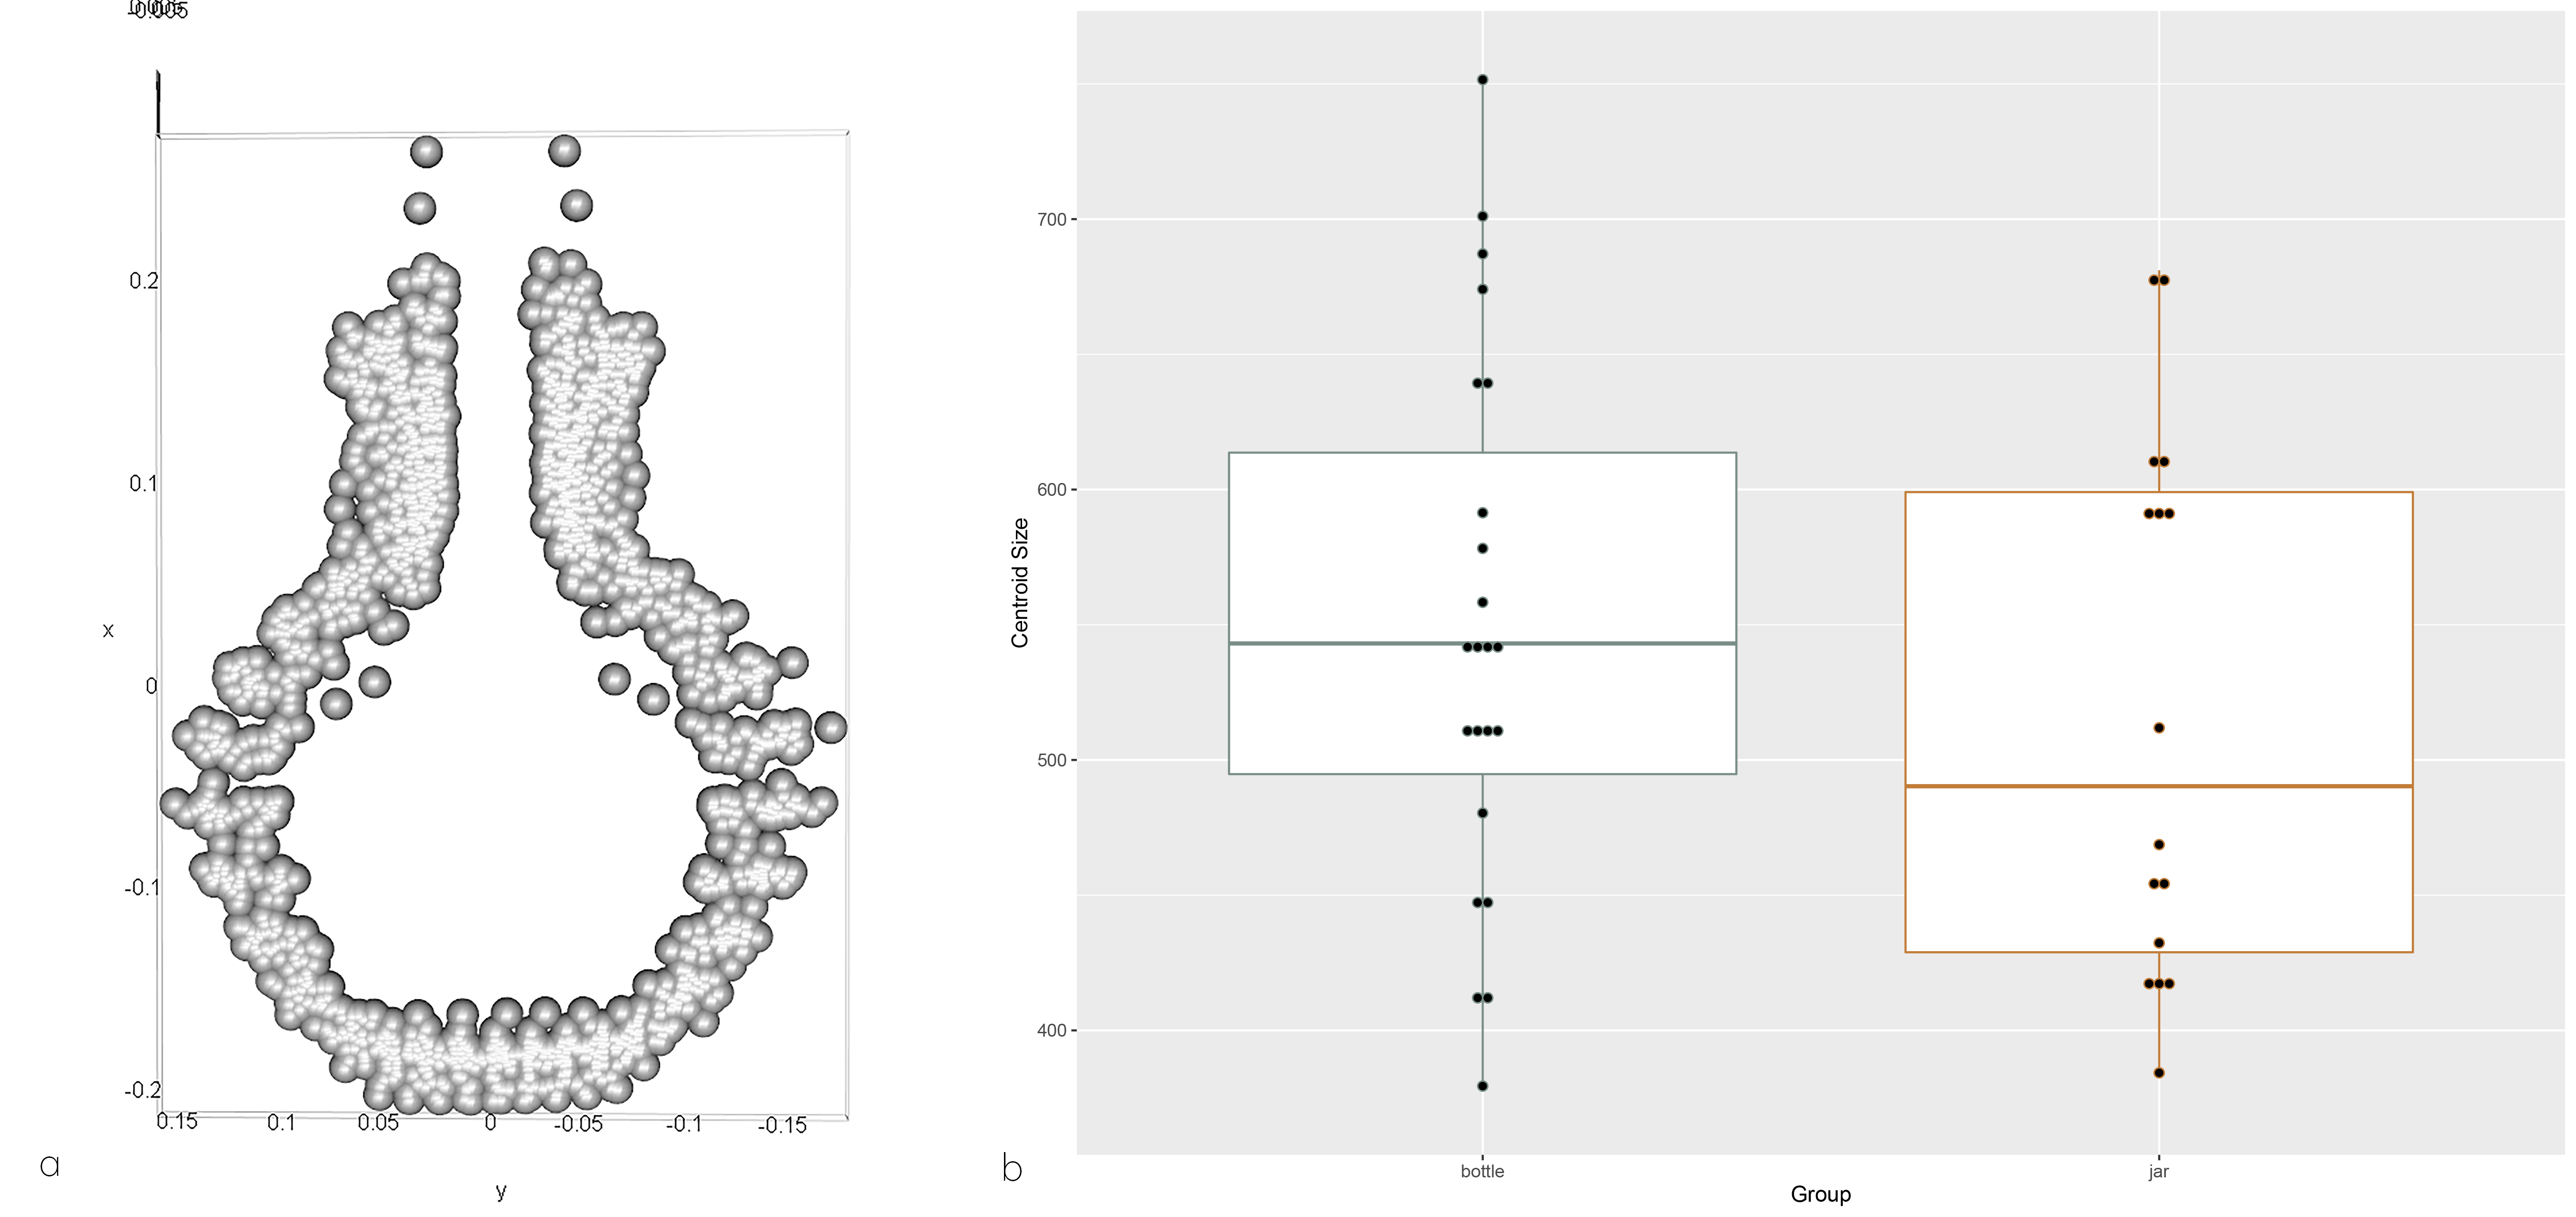
\includegraphics[width=\linewidth]{figs/gpa.csize.png}
\caption{Results of a, generalised Procrustes analysis; and b, boxplot of centroid sizes for Chimu bottles (gray) and jars (orange).}
\label{fig:gpa}
\end{figure}

\hypertarget{principal-components-analysis}{%
\subsubsection{Principal Components
Analysis}\label{principal-components-analysis}}

Principal components analysis \citep{RN1746} was used to visualise shape
variation among the elliptical bifaces, and the scatterplot and convex
hulls represent the dispersion of shapes in tangent space (Figure
\ref{fig:pca}) \citep{RN8633,RN5616,RN11143,RN7550}. The shape ranges
described by each principal axis is commonly visualized using thin-plate
spline warping of a reference image \citep{RN1731,RN479}.

\begin{figure}\centering
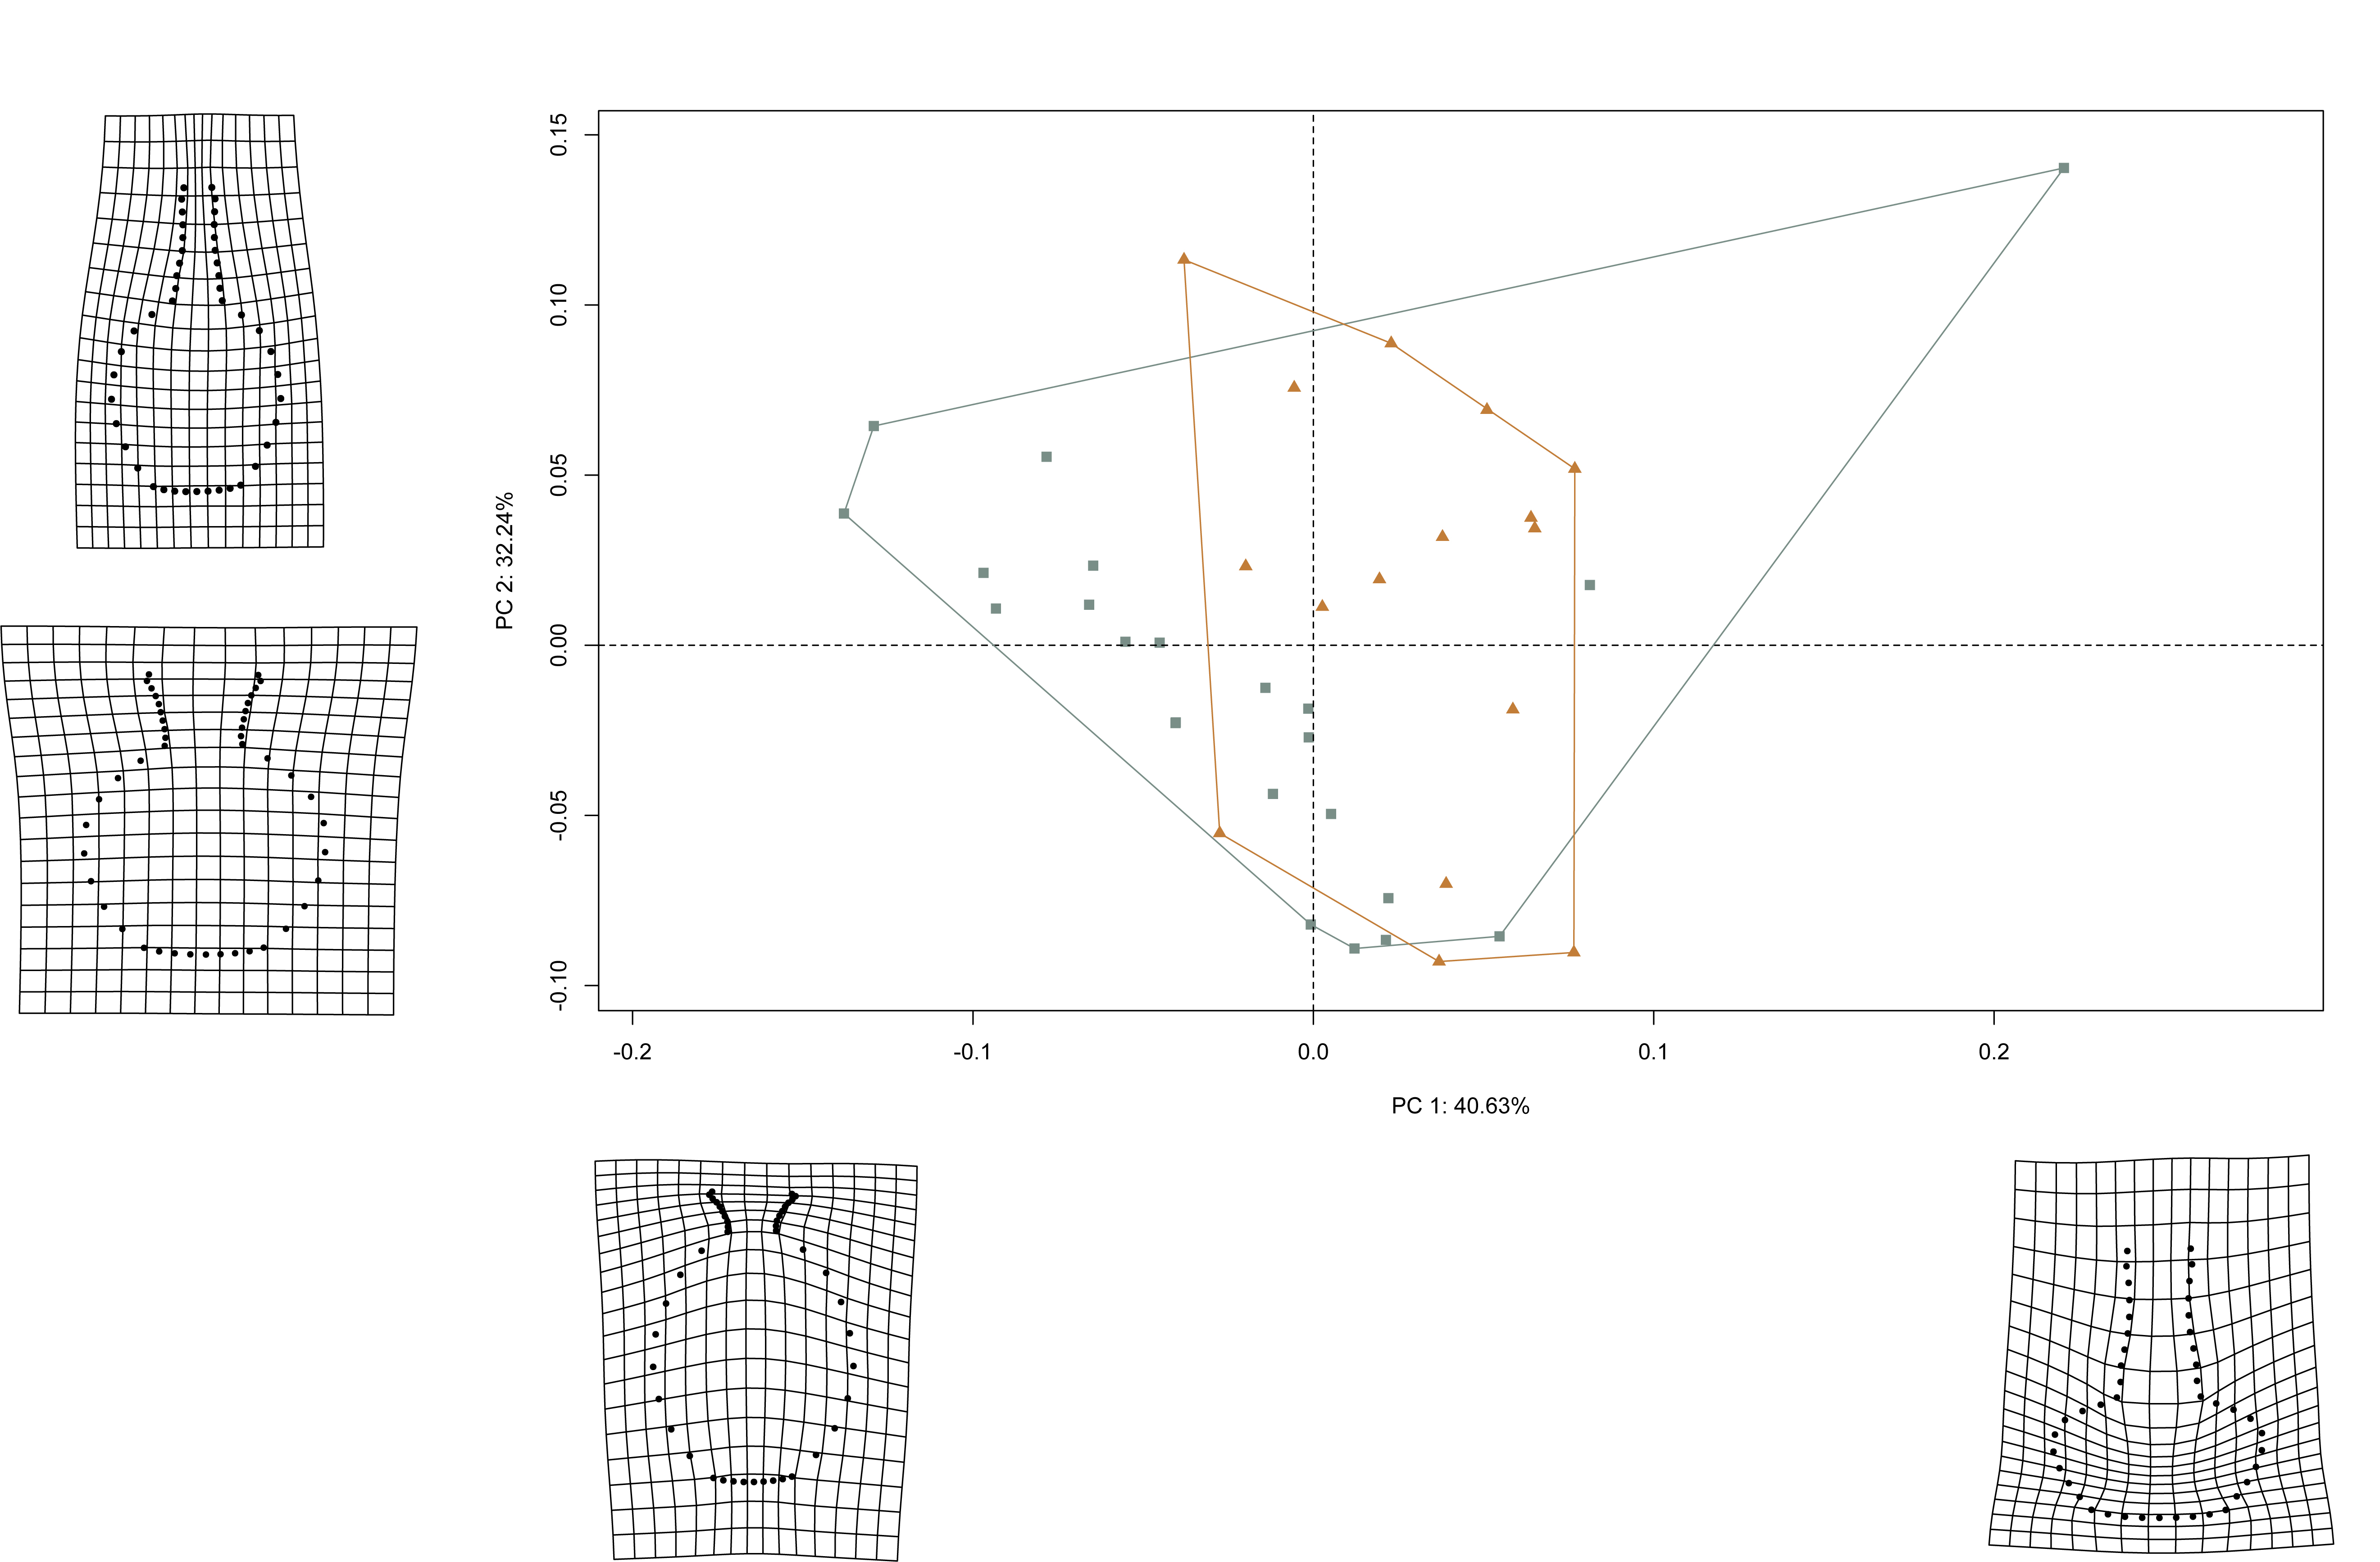
\includegraphics[width=\linewidth]{figs/pca-warp-botjar.jpg}
\caption{PCA summarizing shape variation for Chimu bottles (gray) and jars (orange). }
\label{fig:pca}
\end{figure}

\hypertarget{procrustes-anovas}{%
\subsubsection{Procrustes ANOVAs}\label{procrustes-anovas}}

To assess whether shape changes with size (allometry), and whether shape
and size differed by group (bottles and jars), Procrustes ANOVAs
\citep{RN1749} were run that enlist effect-sizes (zscores) computed as
standard deviates of the generated sampling distributions
\citep{RN1756}. A residual randomization permutation procedure (RRPP; n
= 10,000 permutations) was used for all Procrustes ANOVAs
\citep{RN1655,RN11775}, which has higher statistical power and a greater
ability to identify patterns in the data should they be present
\citep{RN1719}.

Vessel shape differs significantly between bottles and jars
(RRPP=10,000, Rsq=0.0974, Pr(\textgreater F) = 0.0035); however, vessel
size does not (Figure \ref{fig:mshape})
(\href{https://seldenlab.github.io/peru.bottle.jar/}{Supplementary
Materials, Ch. 4}). A subsequent analysis of bottle neck/rim and
body/base morphology demonstrated that while the neck/rim of Chimu
bottles and jars differs significantly in shape (RRPP = 10,000, Rsq =
0.27367, Pr(\textgreater F) = 0.0005), body/base shape remains
consistent (Figure \ref{fig:mshape})
(\href{https://seldenlab.github.io/peru.bottle.jar/}{Supplementary
Materials, Ch. 5}).

\begin{figure}\centering
\includegraphics[width=\linewidth]{figs/mshape.compare.png}
\caption{Means shapes and comparisons for Chimu bottles and jars, as well as necks and rims. }
\label{fig:mshape}
\end{figure}

\hypertarget{discussion}{%
\section{Discussion}\label{discussion}}

Linear measurements from the sample of jars and bottles included vessel
height, rim thickness, and the diameter of each vessel at its orifice,
neck, belly, and base. Of these metrics, vessel height, base diameter,
and neck diameter did not differ significantly between the two samples.
Overall, the jars and bottles in our pilot sample overlap in some key
dimensions, with the bottles showing greater overall size variations,
which would be not be consistent with production using a single set of
molds. The other three sets of linear measurements showed significant
differences between the jars and bottles in our sample, in terms of
orifice diameter, belly diameter, and rim thickness. Given the different
production scenarios emerging from archaeological field analyses---a
combination of hand-shaping and use of whole vessel or elemental molds,
the significant differences in orifice and belly diameters might
indicate that the kinds of bottles and jars in our sample were produced
as distinct shapes, rather than by mixing and matching different molds
to cater to changing consumer tastes. The differences in rim thickness
suggest that distinct production practices were used when producing
bottles and jars. {[}\emph{\textbf{Zac: Should we discuss the analysis
of the figures on the vessels, and then point out that it's
inconclusive, or just leave that out?}}{]}

The analysis of whole vessel morphology revealed that there was no
significant difference in size between the jars and bottles in our
sample. There is considerable size difference within both vessel
categories, a variation that would argue against widespread use of the
same vessel molds. Given the diverse and uncertain provenance of the
vessels in the sample, this is not necessarily unexpected, and a broader
analysis is still needed. Although our sample of bottles and jars
overlaps in size, the analysis of whole vessel morphology demonstrates
that they differ significantly in shape. This reinforces the
interpretation that these jars and bottles represent distinct vessel
shapes, although exploring the significance of that distinction (e.g.,
different social functions, or production at different places or times)
would require a larger vessel sample.

Given the possibility that the selected bottles and jars could have been
produced using either whole-vessel or partial molds, we focused the 3D
analysis onto neck and basal morphology. PCA results for both revealed
significant differences between the two vessel shapes. While bottle and
jar necks are of similar diameters where they attach to the vessel body,
bottle necks flare outward at their orifice, whereas jars maintain a
vertical or slightly narrowing spout. Analysis of basal shape had
comparable results: there was no significant difference in the sizes of
bottle and jar bases, but the basal shape is significantly different
between the two vessel types. Jar bases are significantly more rounded
than the flat bottle bases. The analysis of these two vessel elements
indicates that the morphological distinctions between bottles and jars
derive from more than one vessel element. The results do not answer the
question of how molds were used to produce these vessels, although they
reinforce the picture that these vessels were produced as distinct
shapes. That is, instead of hand-shaping the vessel bodies (or making
them from a common press-mold) and adding distinctive mold-made necks
and spouts to them, potters produced vessel bodies and necks in ways
that kept the distinction between bottles and jars.

\hypertarget{conclusions}{%
\section{Conclusions}\label{conclusions}}

Our first stage of GM analysis of Chimú blackware pottery confirms that
high-resolution scanning and morphological analysis of whole vessels and
key vessel elements is feasible for some of the common vessel categories
found in the Chimú assemblage. Data collection proved to be logistically
straightforward, and our work with publicly-held collections provided
opportunities for public education and outreach, enhancing the ethical
dimensions of the new research. The morphological analysis of whole
vessels presented some challenges for working with some of the more
complex shapes that appear in the Chimú assemblage, but we found bottles
and jars to be amenable to analysis and abundant enough to build
sizeable samples for further analysis.

The morphological comparison of bottles and jars from the AAHC revealed
features that were significantly different between the two shape
classes. Although of similar sizes, the bottles and jars in our sample
were distinguishable as whole vessels, and their basal and neck shapes
were significantly different, as were their rim thicknesses. These
results do not resolve the broader questions about workshop practices
that excavators have posed, but they suggest that the bottles and jars
in our sample were produced as distinct vessels, rather than using
common press molds to produce some elements (e.g., vessel bodies), or
``mixing and matching'' molded elements in a way that would make the two
shapes harder to distinguish morphologically. By broadening our study to
include bottles and jars from the AMNH, we can consider additional
characteristics of these vessels, including size differences and the use
of modeled adornments (of plants, animals, and humans) on the vessels.
Such work will bring us closer to explaining key elements of Chimú
ceramic variation over time, and in different parts of the north coast,
offering welcome insights into the economic organization of the Chimú
Empire.

\hypertarget{acknowledgments}{%
\subsection{Acknowledgments}\label{acknowledgments}}

We extend our gratitude to\ldots{}

\hypertarget{funding}{%
\subsection{Funding}\label{funding}}

Components of this analytical work flow were developed and funded by a
Preservation Technology and Training grant (P14AP00138) to RZS from the
National Center for Preservation Technology and Training (NCPTT), and
additional grants to RZS from the Caddo Nation of Oklahoma and the
National Forests and Grasslands in Texas (15-PA-11081300-033), and the
United States Forest Service (20-PA-11081300-074). Funding to scan the
Chimú vessels in the Art and Art History Collections at The University
of Texas at Austin was provided by The University of Texas at Austin,
with additional support provided by the Heritage Research Center at
Stephen F. Austin State University.

\hypertarget{data-management}{%
\subsection{Data management}\label{data-management}}

All data and analysis code associated with this project can be accessed
through this document or the
\href{https://seldenlab.github.io/anthro.zoo/}{GitHub} repository, which
is digitally curated on the Open Science Framework
(\href{https://osf.io/vzhjr/}{DOI 10.17605/OSF.IO/VZHJR}). The
reproducible nature of this undertaking provides a means for others to
critically assess and evaluate the various analyses
\citep{RN20915,RN20916,RN20917}, which is a necessary requirement for
the production of reliable knowledge.

Reproducibility projects in \href{https://osf.io/ezcuj/}{psychology} and
\href{https://www.cos.io/rpcb}{cancer biology} are impacting current
research practices across all domains. Examples of reproducible research
are becoming more abundant in archaeology
\citep{RN20804,RN21009,RN21001,RN9364,RN11264}, and the next generation
of archaeologists are learning those tools and methods needed to
reproduce and/or replicate research results \citep{RN21007}.
Reproducible and replicable research work flows are often employed at
the highest levels of humanities-based inquiries to mitigate concern or
doubt regarding proper execution, and is of particular import should the
results have---explicitly or implicitly---a major impact on scientific
progress \citep{RN21008}.

\bibliographystyle{tfcad}
\bibliography{interactcadsample.bib}


\input{"appendix.tex"}



\end{document}
